\chapter{RRT}\label{chap:RRT}

\section{General}

The goal of this Thesis was not only to generate a numerical stable, snap optimized polynomial trajectory but also to explore a dense (indoor) environment and plan an aggressive trajectory in between the obstacles. Hence, the Rapidly-Exploring Random Tree (RRT) algorithm is used to find a collision free straight-line solution through dense environments. The sampling points oft the RRT (or RRT*) algorithm are then used as the vertices in the polynomial optimization.


\section{RRT Algorithm}\label{sec:RRT}

RRT is a computational efficient algorithm to find a path in a high dimensional space by randomly building a space-filling tree. The sampling points are drawn randomly from the sample space and the tree grows incrementally. 
For each new sample the algorithm attempts to build a collision-free connection to the nearest state in the tree. If a collision-free connection is possible the sample and the connection are added to the tree. \newline

An iteration of the RRT algorithm can be depicted schematically:


\begin{enumerate}
  \item Generate a random sample
  \item Find nearest state in tree
  \item Try to build a collision-free connection to the nearest state
  \item If feasible, add the sampled state and the connection to the tree
\end{enumerate}

\subsection{Goal State}

As mentioned above, the RRT algorithm is based on random samples. Therefore it is very unlikely that a sampled state perfectly matches the desired goal state. \newline

There are two different strategies to enable the RRT algorithm to get to the goal. One strategy is to define not only a goal state but a goal region. Every random sample which is located within the goal region is considered a goal state. As soon as a collision-free connection to a sample in the goal region is established, this trajectory is stored as the best trajectory. At this point the algorithm can be stopped or further iteration can be performed to find a better trajectory to the goal region. Once an other state from the goal region is sampled and the cost of the path to the new state is lower then the cost of the best trajectory, the best trajectory is replaced by the new path. \newline
Another strategy is to steer the RRT algorithm directly to the goal state. In addition to the randomly sampled states the exact goal state is added to the algorithm. The schematic description of an iteration of the RRT algorithm listed in section \ref{sec:RRT} can be modified to represent an iteration with the goal state:

\begin{enumerate}
  \item Insert goal state
  \item Find nearest state in tree
  \item Try to build a collision-free connection to the nearest state
  \item If feasible, add the sampled state and the connection to the tree
\end{enumerate}

In all the cases where a direct collision-free connection between start and goal state is not possible the iteration with the goal state will not succeed in a first attempt. Hence the iterations with the randomly sampled states described in section \ref{sec:RRT} are needed to build the space filling tree.\newline

Figure \ref{pic:smallGamma} depicts the straight line solution of the RRT algorithm with a fixed goal state. The figure is in bird's eye perspective and shows a crossing of different hallways. The blue cells represents the floor and the green cells represents the walls. The map was generated with a stereo camera and was not reworked. Therefore some of the cells of the floor which should be occupied/blue are left free. 

\begin{figure}[H]
   \centering
   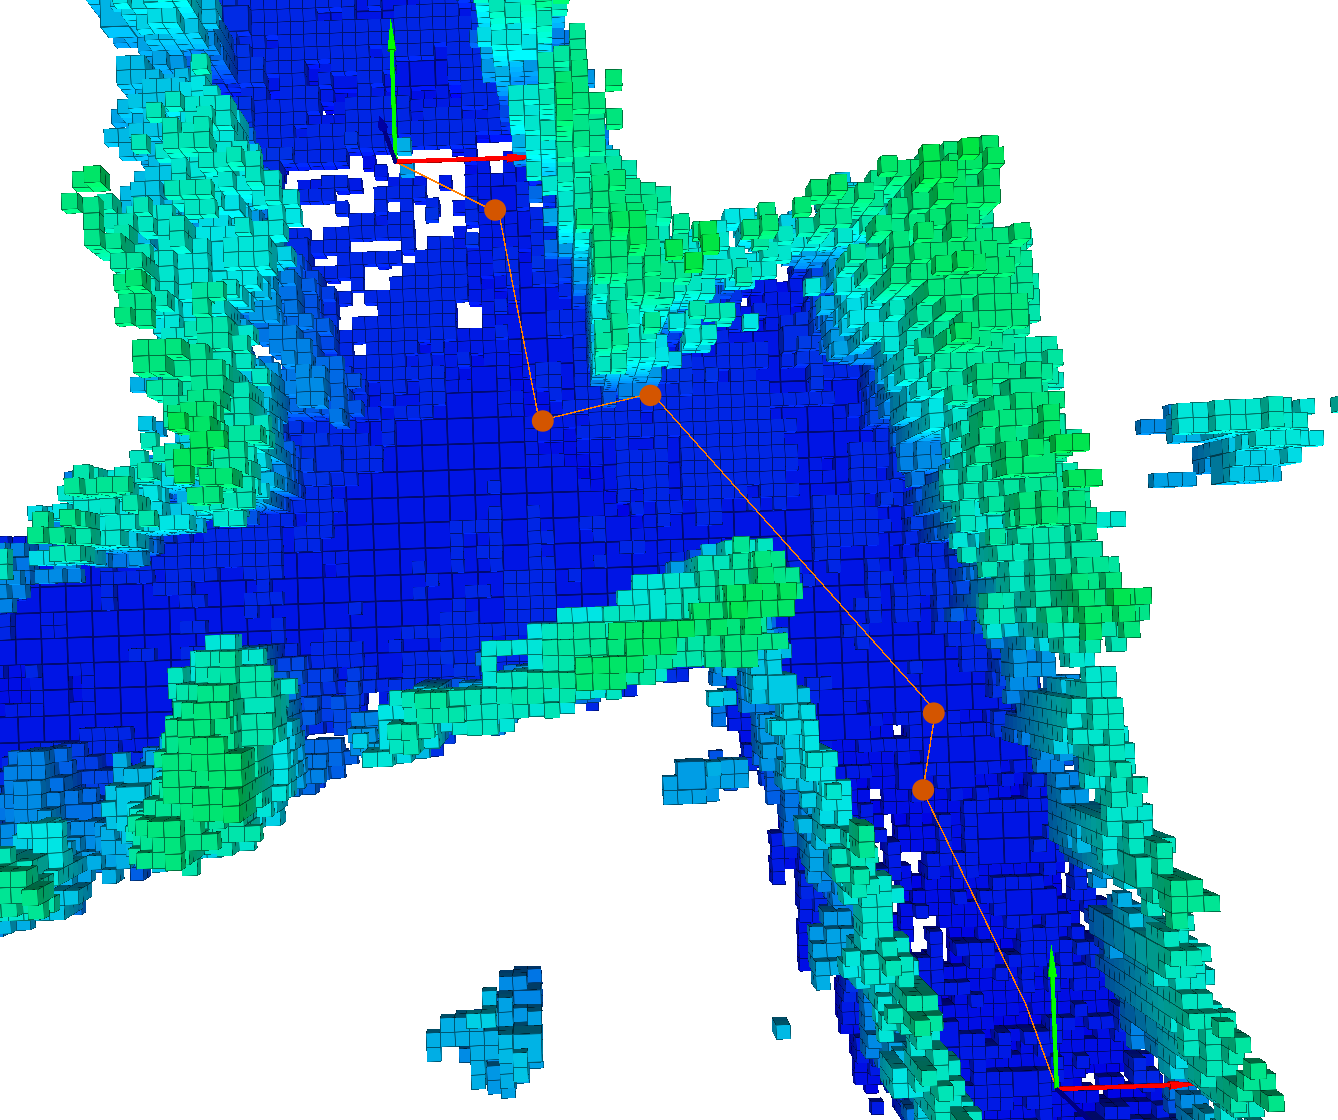
\includegraphics[width=1\textwidth]{pics/smallGammaP.png}
   \caption{Straight line solution of the RRT algorithm with a fixed goal state. Start and goal state are each represented by a red $x$-vector and a green $y$-vector. The random sampled states are depicted as orange dots.}
   \label{pic:smallGamma}
\end{figure}



\section{RRT* Algorithm}\label{sec:RRTstar}

In contrast to the RRT algorithm the RRT* (or RRT Star) algorithm not only tries to connect to the nearest state in the tree but to several states near the sampled state. The user can define a threshold (on the distance) which defines which states of the tree belongs to the "near states". If there is no state within the user specified range the algorithm attempts to build a collision-free connection to the nearest state in the tree just as the RRT algorithm.  \newline
As a first step, the sampled state is connected to the best state among the near states whereas best means minimum cost/distance. Once the sampled state is added to the tree all the other states among the set of near states are connected to the sampled state. If the connection is collision-free and the cost of the total path is smaller than the cost of the existing path, the old path is replaced. \newline

An iteration of the RRT* algorithm can be depicted schematically:


\begin{enumerate}
  \item Generate a random sample
  \item A threshold defines a set of near states
  \item Try to build a collision-free connection to best state among the near states
  \item Add the sampled state and the connection to the tree 
  \item Try to connect all the other states from the set with the sampled state 
  \item Replace the old path if the new one has a smaller cost
  \item If there is no near state within the threshold apply the RRT algorithm
\end{enumerate}


Because the RRT* algorithm tries to connect to several states each iteration, the procedure of finding a path takes longer and is computationally more expensive. However, solution with lower cost can be found which is more important for most real life applications.

\subsection{Rewiring}

The sequence of step 5 and step 6 of the RRT* algorithm ("Try to connect all the other states from the set with the sampled state", "Replace the old path if the new one has a smaller cost") are called "rewiring". \newline 
The threshold which defines the set of near states depends on a user specified parameter $\gamma$. In this case, the threshold is the radius of a sphere, i.e. all the near states are located within this sphere. The radius $r$ can be calculated according to


\begin{equation}
r = \gamma * \left(\frac{ln(n+1)}{n+1}\right)^{1/d}
\label{equ:ballradius}
\end{equation}

where $n$ is the number of states which are already in the tree. The dimension of the state space $d$ is a fixed parameter and $ln$ represents the natural logarithm.\newline

As mention in section \ref{sec:RRTstar} the RRT* algorithm is computationally more expensive but returns trajectory with lower cost. Both aspects are caused by the rewiring and are therefore strongly influenced by the parameter $\gamma$. A large $\gamma$ defines a large sphere, hence it is likely to have more states (which are already in the tree) to be located within the sphere. The rewiring of the near states tends to result in shorter trajectories with fewer segments.

Figure \ref{pic:smallBBX} depicts the straight line solution of the RRT* algorithm with a fixed goal state. Compared to figure \ref{pic:smallGamma} a superior trajectory is found since a rewiring of the states in the tree was performed.

\begin{figure}[H]
   \centering
   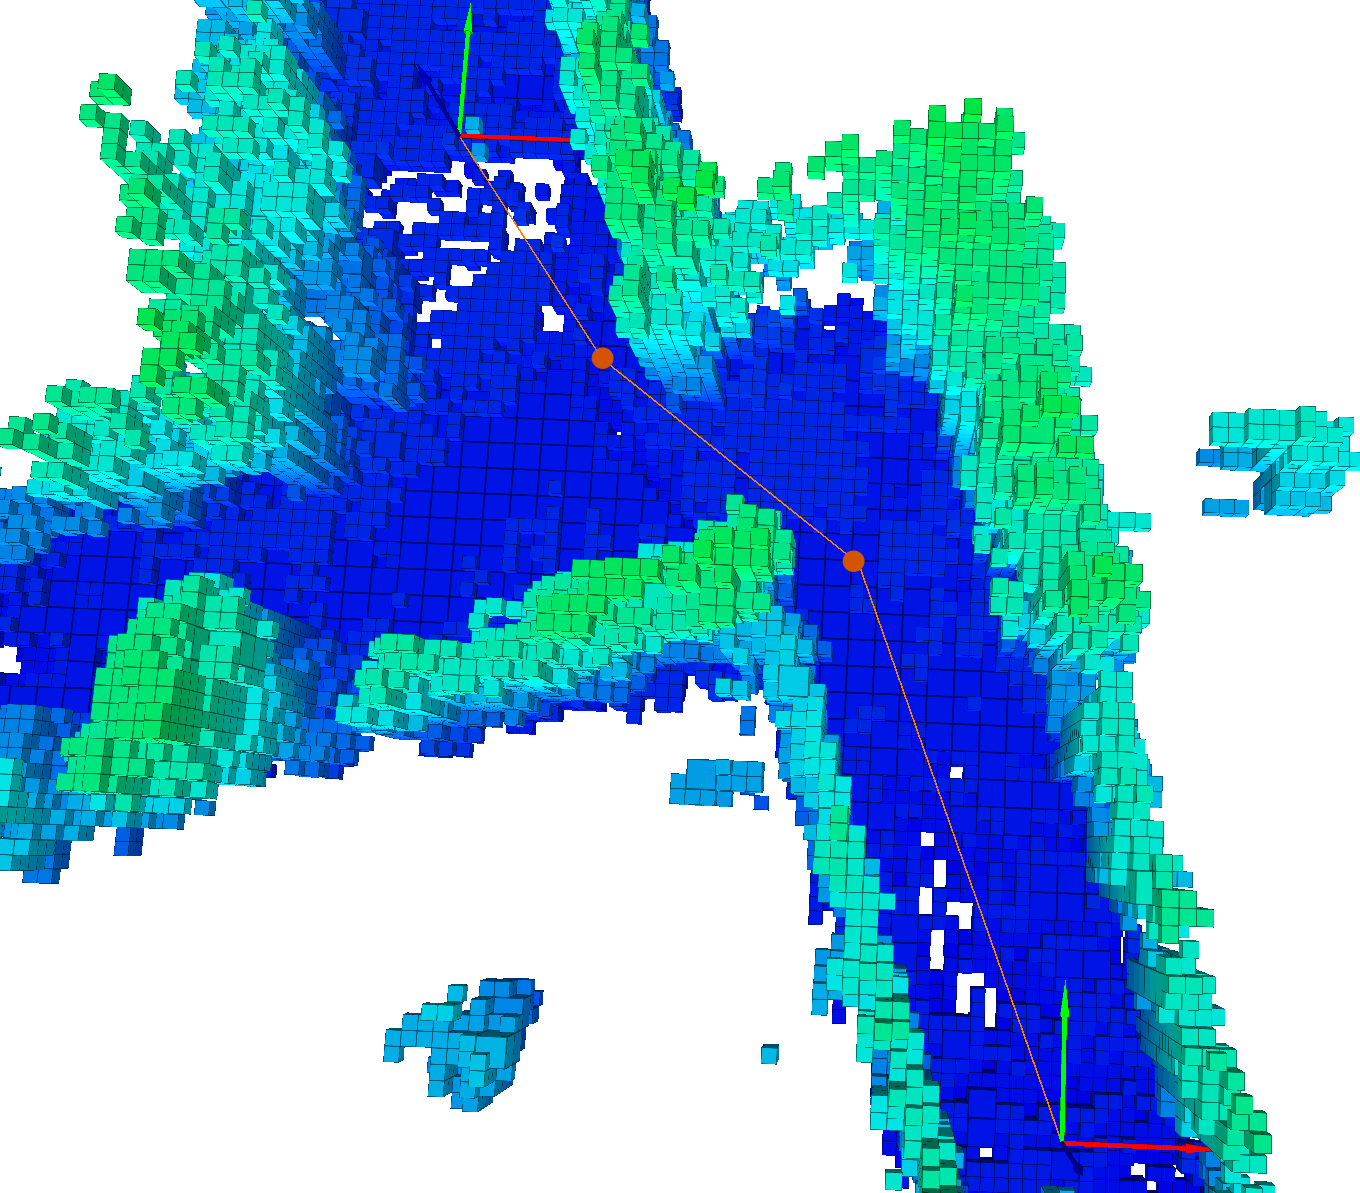
\includegraphics[width=1\textwidth]{pics/smallBBXP.png}
   \caption{Straight line solution of the RRT* algorithm with a fixed goal state. Start and goal state are each represented by a red $x$-vector and a green $y$-vector. The random sampled states are depicted as orange dots. The $\gamma$ parameter in this example was set to $\gamma = 1.5$.}
   \label{pic:smallBBX}
\end{figure}


\subsection{Bounding Box}

The straight line solution in figure \ref{pic:smallBBX} is collision-free but passes by very close to the walls. In real life application not only a point mass but a object (in this master thesis a UAV) should follow the trajectory. Therefore a bounding box is installed around the trajectory. \newline
The bounding box is implemented as a cuboid. The 3 dimension of the cuboid can be defined individually. The trajectory is then divided into a discrete trajectory and the bounding box is installed around the discrete points. If there is a obstacle in one of the bounding boxes the hole straight line is considered as  in collision. \newline

Figure \ref{pic:bbx} depicts the straight line solution of the RRT* algorithm with a bounding box. In contrast to figure \ref{pic:smallBBX} the trajectory is now located more central in the hallway because the bounding box makes it impossible to pass by the wall very close. Because the trajectory proceeds less direct from start to goal state the total distance of the trajectory increases. Although the the number of segments increases as well from 3 segments in figure \ref{pic:smallBBX} to 4 segments in figure \ref{pic:bbx} this is not necessarily a consequence of the bounding box. Performing additional iterations (including more sampling points and more rewiring) could lead to a solution with 3 segments.

\begin{figure}[H]
   \centering
   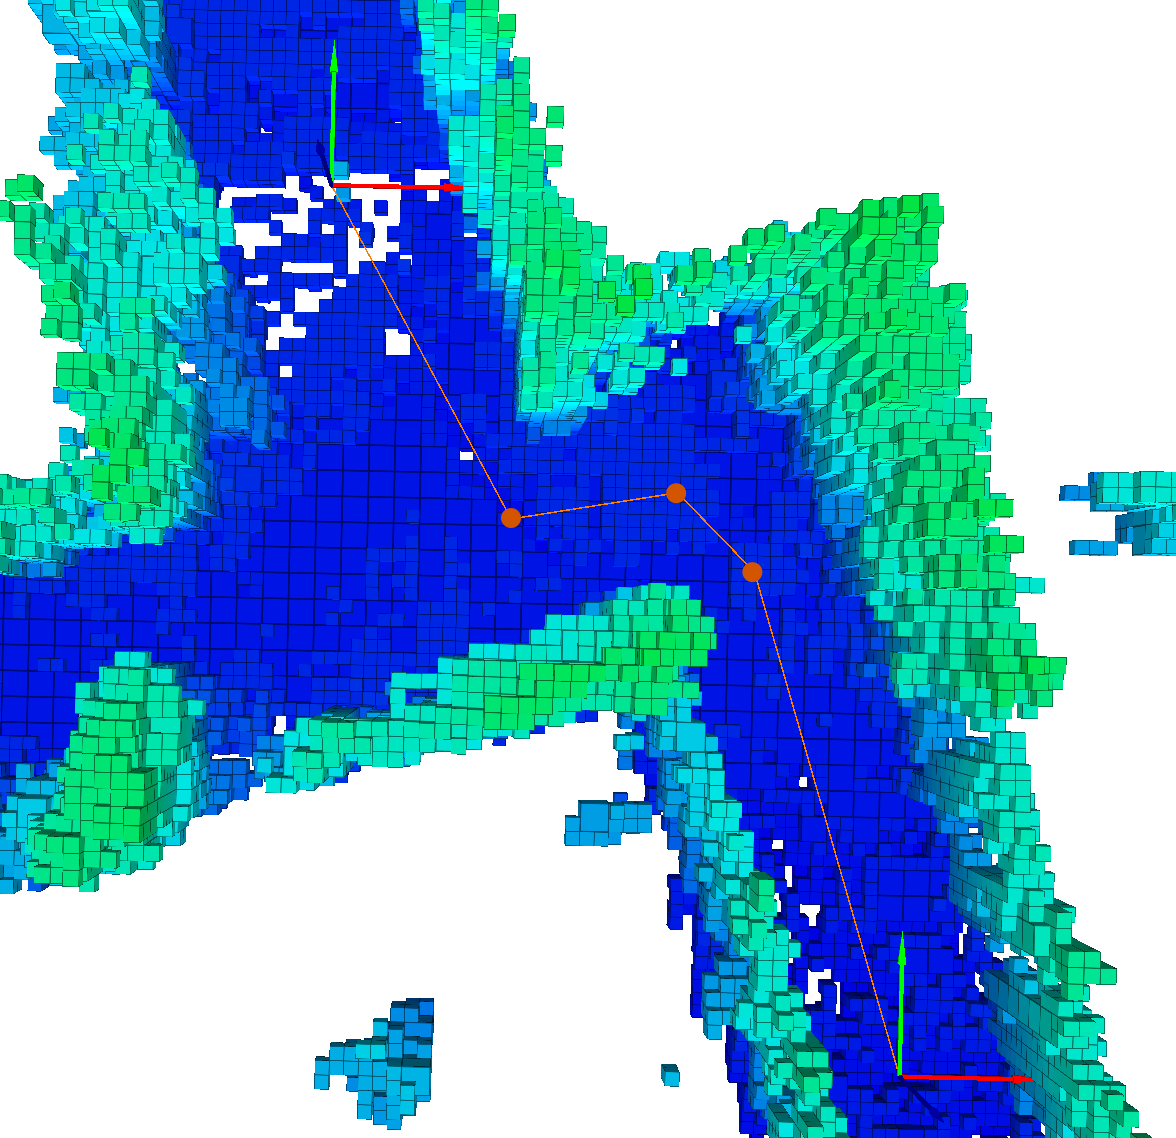
\includegraphics[width=1\textwidth]{pics/extensionLongP.png}
   \caption{Straight line solution of the RRT* algorithm with bounding box. Due to the bounding box the trajectory is located more central in the hallway because the bounding box makes it impossible to pass by the wall very close. The $\gamma$ parameter in this example was set to $\gamma = 1.5$.}
   \label{pic:bbx}
\end{figure}

\subsection{Ray Check}

 TODO: verbindung zu Octompa
 
 matlab figure



%\begin{figure}[h]
%   \centering
%   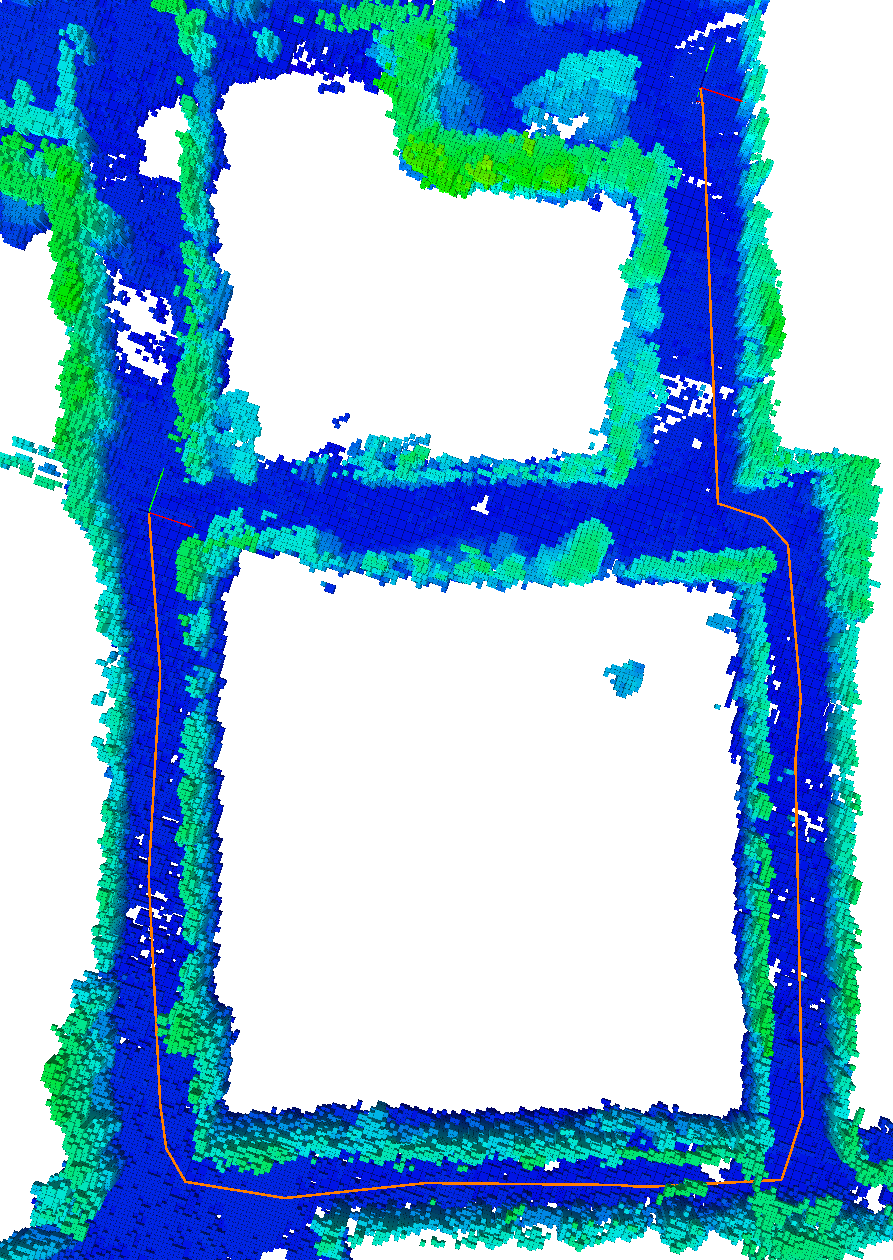
\includegraphics[width=1\textwidth]{pics/MapLine.png}
%   \caption{Ein Bild.}
%\end{figure}



%\begin{figure}[h]
%   \centering
%   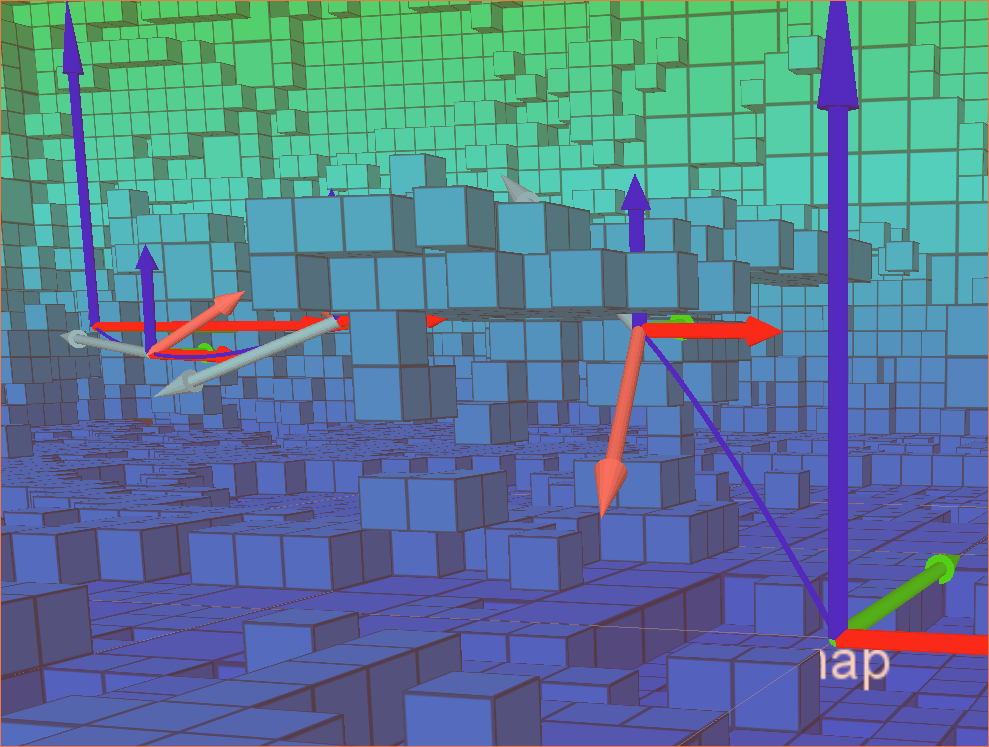
\includegraphics[width=1\textwidth]{pics/initialSolution.png}
%   \caption{Ein Bild.}
%\end{figure}
%
%
%\begin{figure}[h]
%   \centering
%   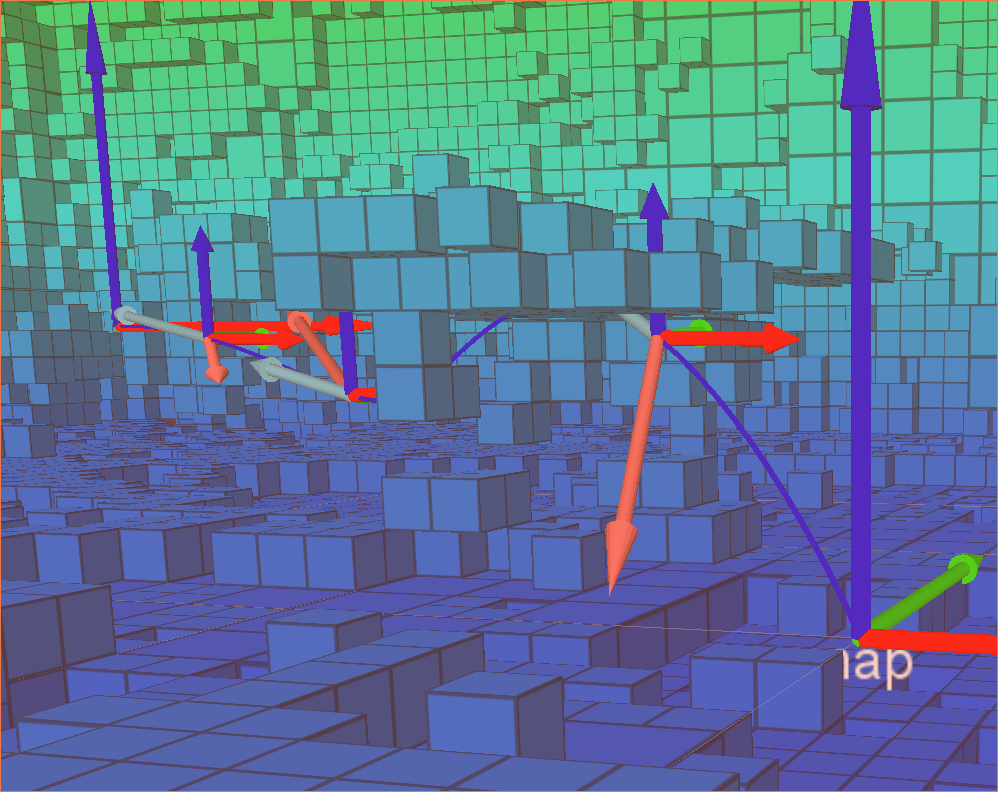
\includegraphics[width=1\textwidth]{pics/Vertex_in_middle_2.png}
%   \caption{Ein Bild.}
%\end{figure}
%
%\begin{figure}[h]
%   \centering
%   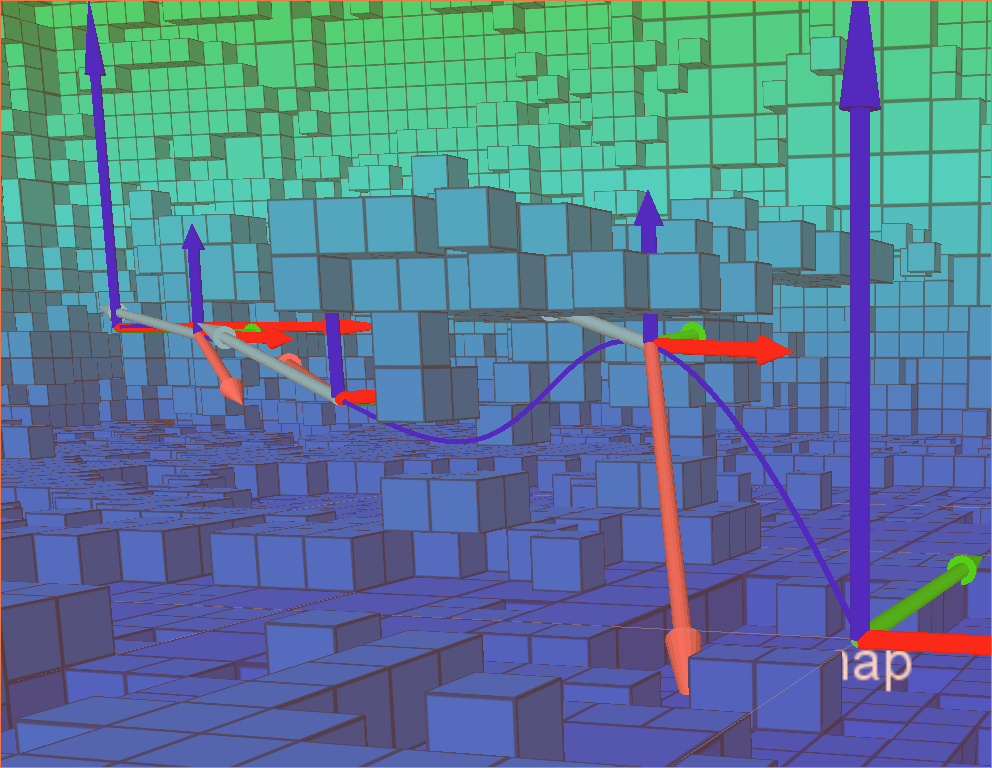
\includegraphics[width=1\textwidth]{pics/section.png}
%   \caption{Ein Bild.}
%\end{figure}
%
%
%\begin{figure}[h]
%   \centering
%   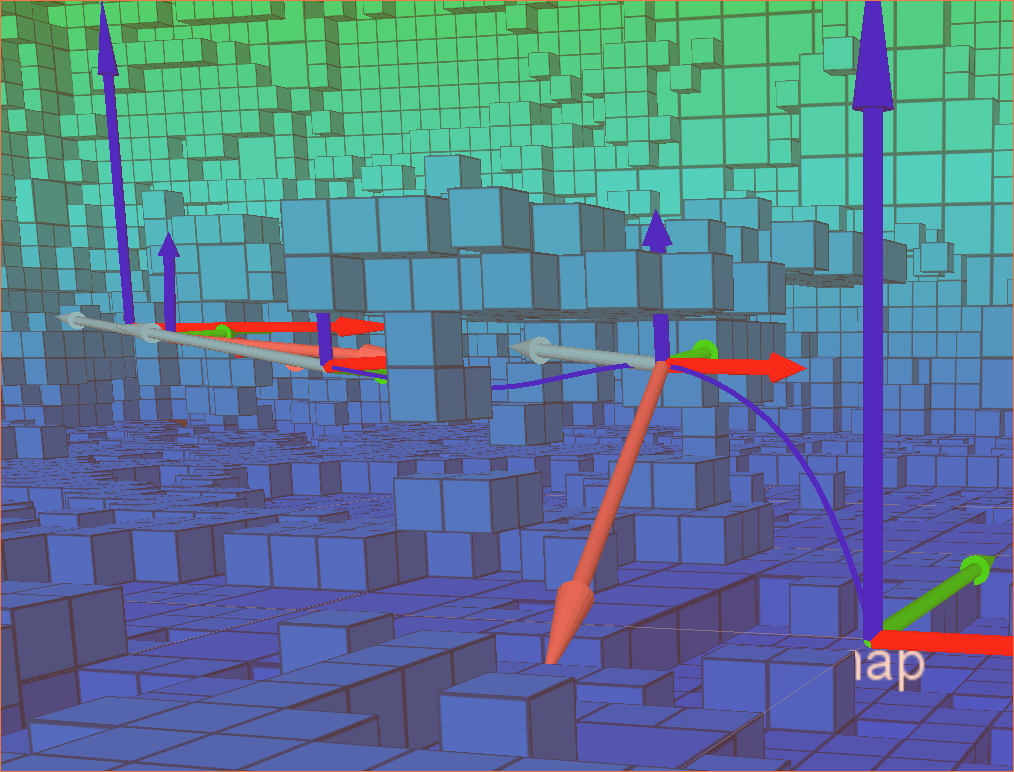
\includegraphics[width=1\textwidth]{pics/Nlopt_after_sectionAndTime.png}
%   \caption{Ein Bild.}
%\end{figure}